\documentclass[a4paper]{beamer}

\usepackage{polski}
\usepackage[utf8]{inputenc}
\usepackage{amsmath}
\usepackage{amssymb}
\usepackage{enumerate}
\usepackage{hyperref}
\usepackage{listings}
\usepackage{graphicx}
\usepackage{color}

\graphicspath{ {./images/} }
\usetheme{Warsaw}
\useoutertheme{infolines}
\setbeamertemplate{footline}{}
\setbeamertemplate{headline}
{
\begin{beamercolorbox}{section in head/foot}
\vskip2pt\insertnavigation{\paperwidth}\vskip2pt
\end{beamercolorbox}%
}

\DeclareGraphicsExtensions{.png}

\author{Agnieszka Pocha \\ Michał Kowalik}
\title{Klątwa wielowymiarowości \\ The Curse of Dimensionality}
\date{11 marca 2015}

\begin {document}


\begin{frame}
\titlepage
{\footnotesize
na podstawie książki: \\
Bertrand Clarke, Ernest Fokoue, Hao Helen Zhang \\
}
\textit{Principles and Theory for Data Mining and Machine Learning}
\end{frame}


\begin{frame}
\frametitle{Agenda}
\tableofcontents
\end{frame}

\section{AI, ML, Data Mining}
\begin{frame}
\begin{block}{Sztuczna Inteligencja - AI}
\textit{W świecie, gdzie niepewność modelu jest często ograniczeniem w procedurach wnioskowania, ważniejszym stała się predykcja/przewidywanie niż testowanie czy estymacja.}... \\
Dział informatyki zajmujący się rozwiązywaniem problemów, które nie są efektywnie algorytmizowalne.
\end{block}
\pause
\begin{block}{Uczenie Maszynowe - Machine Learning}
Pojęcie odnosi się do użycia formalnych struktur (maszyny) do wnioskowania (uczenie) - MODELOWANIE. Informacja tutaj pomaga zmniejszyć niepewność.
\end{block}
\pause
\begin{block}{Data Mining}
Odnosi się do przeszukiwania ogromnych, wielowymiarowych, wielotypowych zbiorów danych. Informacje są nieustrukturyzowane i wielorakie.
\end{block}
\end{frame}
\begin{frame}

\begin{center}
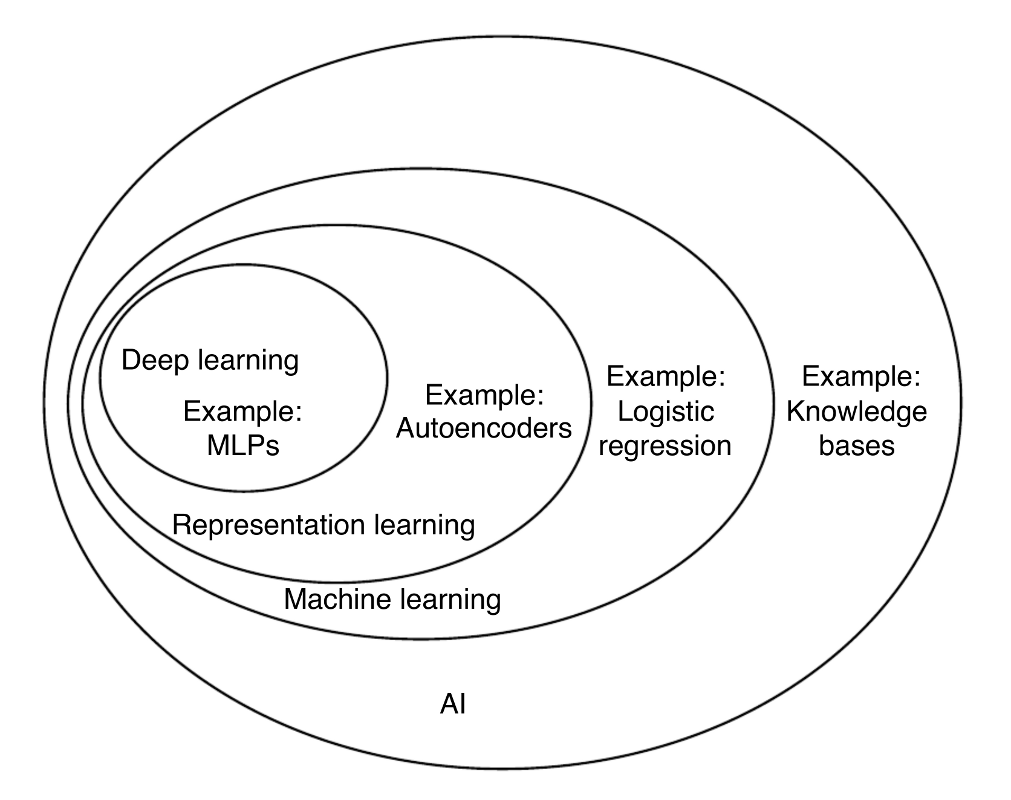
\includegraphics[height=8cm]{aiclasification.png}
\end{center}
\end{frame}

\begin{frame}
\begin{block}{Model}
\begin{itemize}
\item Odwzorowanie rzeczywistości
\item $s = v \cdot t$
\end{itemize}
\end{block}
\pause
\begin{block}{Przestrzeń}
Przestrzeń – zbiór, w którym określone są rozmaite relacje i działania pomiędzy jego elementami
\end{block}
\begin{block}{Metryka}
Metryką (w zbiorze X) nazywa się funkcję: \\
$d: X \times X \to [0, +\infty),$
która dla dowolnych elementów a, b, c tego zbioru spełnia następujące warunki:
\begin{itemize}
\item identyczność nierozróżnialnych: $d(a, b) = 0 \iff a = b$
\item symetria: $d(a, b) = d(b, a)$
\item warunek trójkąta: $d(a, b) \leqslant d(a, c) + d(c, b)$
\end{itemize}
Gdy d jest metryką w zbiorze X, to para (X, d) nazywana jest przestrzenią metryczną
\end{block}
\end{frame}
\begin{frame}
\begin{block}{Metryka Euklidesowa}
Ogólnie, w przestrzeni $\mathbb R^n$ metrykę euklidesową definiuje się wzorem:
$$d_e(\mathbf x, \mathbf y) = \sqrt{(y_1 - x_1)^2 + \dots + (y_n - x_n)^2}$$
tzn. jako pierwiastek euklidesowego iloczynu skalarnego różnicy dwóch wektorów przez siebie:
$$d_e(\mathbf x, \mathbf y) = \sqrt{\langle \mathbf y - \mathbf x, \mathbf y - \mathbf x \rangle}$$
\end{block}
\pause
\begin{block}{Metryka Jaccarda}
Metryka używana do porównywania zbiorów:
$J(A,B) = {{|A \cap B|}\over{|A \cup B|}}$ \\
Żeby były spełnione warunki metryki:
$$d_J(A,B) = 1 - J(A,B) = { { |A \cup B| - |A \cap B| } \over |A \cup B| }$$
\end{block}
\end{frame}

\section{Metody Local vs Global}
\begin{frame}
\begin{columns}
\column{.45\textwidth}
\begin{block}{Local Methods}
- K-means \\[0.2cm]
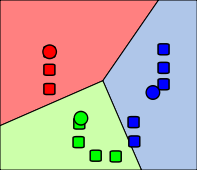
\includegraphics[height=4cm]{kmeans.png}
\end{block}
\column{.45\textwidth}
\begin{block}{Global Methods}
- sieci neuronowe \\[0.2cm]
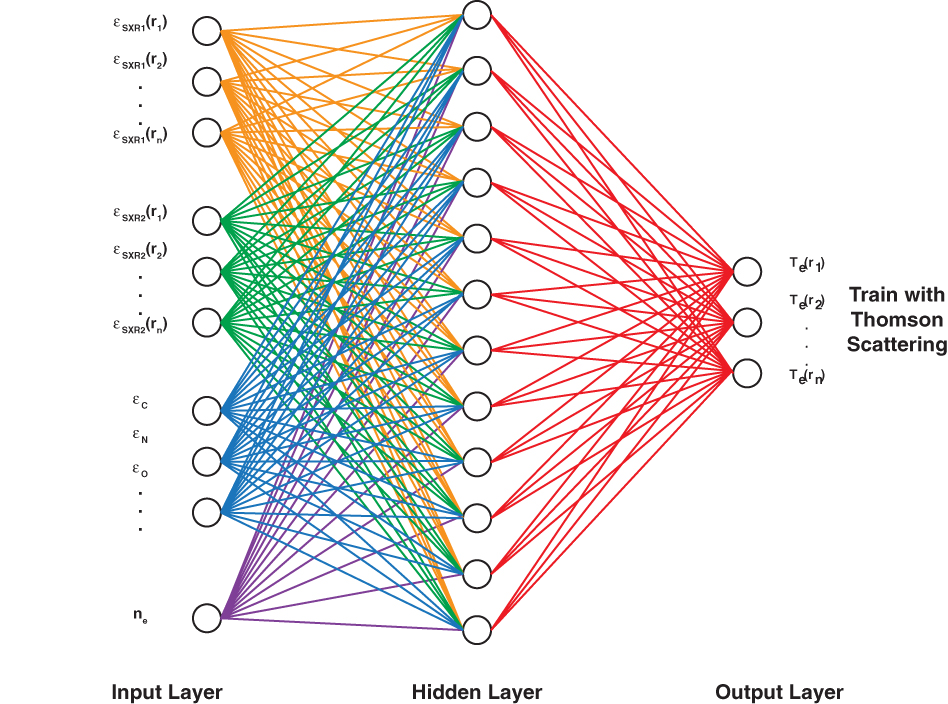
\includegraphics[height=4cm]{neuralnetwork.png}
\end{block}
\end{columns}
\end{frame}

\section{Klątwa wielowymiarowości}
\begin{frame}
\pause
\begin{block}{Intuicja}
Przy wysokim wymiarze przestrzeni, dane są zbyt rzadkie. \\
Przy wysokim wymiarze przestrzeni, liczba możliwych modeli do rozważenia rośnie w sposób super-wykładniczy (superexponential).

\end{block}
Z ekstremalny przypadkiem mamy do czynienia, gdy przestrzeń ma wiele wymiarów $p$, a danych jest niewiele.
\end{frame}

\begin{frame}
\begin{block}{Wprowadzenie pojęć}
\begin{itemize}
\item Rzadkość (Sparsity)
\item Liczba możliwych modeli
\item Concurvity
\end{itemize}
\end{block}

\end{frame}

\section{Rzadkość}
\begin{frame}
\begin{block}{Motywacja}
Jeśli nie ma zbyt wiele obiektów do porównania w sąsiedztwie jakiegoś punktu $x$, wtedy trudno określić jak powinna wyglądać funkcja $f(x)$.
\end{block}
\begin{block}{}
Gdy liczba wymiarów $p$ rośnie, liczba danych lokalnych maleje do 0. 
\end{block}
\begin{block}{}
Objętość kuli o promieniu $r$ maleje do 0, wraz ze wzrostem wymiaru $p$. \\
$V_{n}=\frac { \pi^{\frac{n}{2}}}{\Gamma (\frac{n}{2}+1)}\cdot r^{n} = \begin{cases} \displaystyle {\pi^k\over k!}\cdot r^n & \mbox{dla }n=2k, \\[2ex] \displaystyle {2^k \pi^{k-1}\over n!!}\cdot r^n & \mbox{dla } n=2k-1, \end{cases}$
\end{block}
\end{frame}

\begin{frame}

\begin{center}
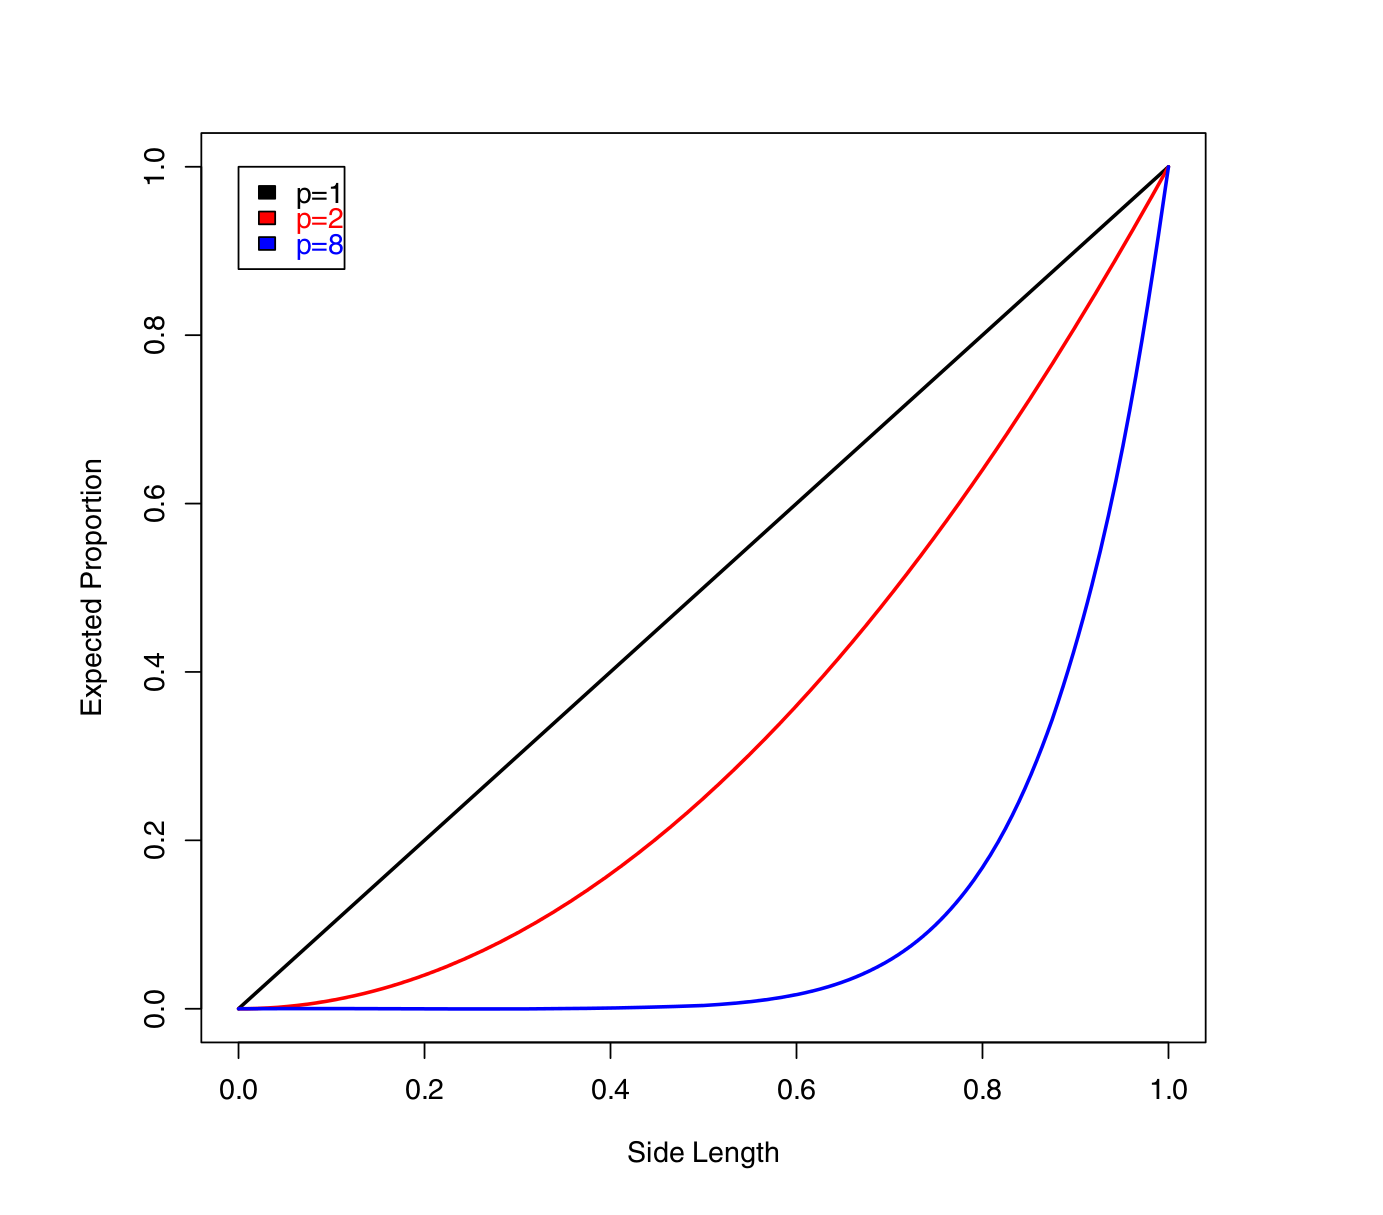
\includegraphics[height=9cm]{ball.png}
\end{center}
\end{frame}


\section{Liczba modeli}
\begin{frame}
\begin{block}{}
Liczba modeli rośnie super-wykładniczo (superexponential) wraz ze wzrostem rozmiaru.
\end{block}
\begin{block}{Przykład}
Dla $p=1$ jest 7 możliwych różnych modeli: \\
$\mathbb{E}(Y) = \beta_0$, \\
$\mathbb{E}(Y) = \beta_0 + \beta_1 x_1$, \\
$\mathbb{E}(Y) = \beta_0 + \beta_1 x_1 + \beta_2 x_1^2$, \\[0.3cm]


$\mathbb{E}(Y) = \beta_1 x_1$, \\
$\mathbb{E}(Y) = \beta_0 + \beta_2 x_1^2$, \\[0.3cm]


$\mathbb{E}(Y) = \beta_2 x_1^2$, \\
$\mathbb{E}(Y) = \beta_1 x_1 + \beta_2 x_1^2$, \\

\end{block}
\begin{block}{}
Dla $p=2$ liczba możliwości wynosi 63.
\end{block}
\begin{block}{}
Oczywistym jest, że problem się pogarsza dla wielomianów większego rzędu.
\end{block}
\end{frame}

% \section{Concurvity}
%\begin{frame}
% \begin{block}{}
% Concurvity
% \end{block}
% \begin{center}
% 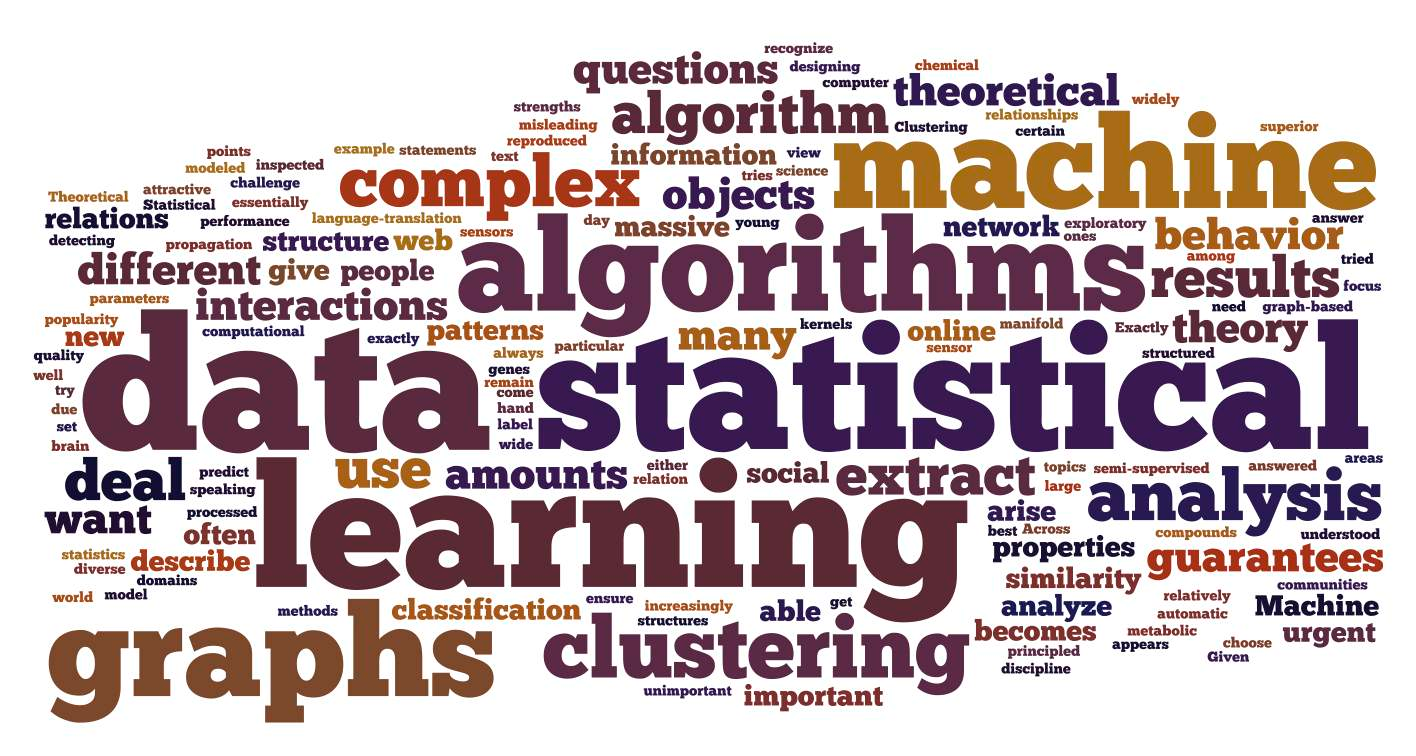
\includegraphics[height=4.5cm]{ml-wordle.png}
% \end{center}
% \end{frame}

\section{Metody radzenia sobie z problemem}
\begin{frame}
\begin{block}{PCA}
Celem PCA jest taki obrót układu współrzędnych, aby maksymalizować w pierwszej kolejności wariancję pierwszej współrzędnej, następnie wariancję drugiej współrzędnej, itd.. \\[0.3cm]
PCA jest często używana do zmniejszania rozmiaru zbioru danych statystycznych, poprzez odrzucenie ostatnich czynników.
\end{block}
\pause
\begin{block}{LDA}
Używanie w uczeniu maszynowym do znalezienia liniowej kombinacji cech, które najlepiej rozróżniają dwie lub więcej klas obiektów lub zdarzeń. Wynikowe kombinacje są używane jako klasyfikator liniowy lub, częściej, służą redukcji wymiarów do późniejszej klasyfikacji statystycznej.
\end{block}
\end{frame}
\end{document}